\chapter{Potential Fields} \label{ch:potential}
\section{Introduction}
Many of the most widely used geophysical methods are governed by a common class of mathematical descriptions known as \emph{potential fields}. Gravity, magnetics, electrostatics, and steady-state heat conduction all fall into this category, despite arising from very different physical processes. What unifies them is not geology, but mathematics: each involves a scalar potential whose spatial variation gives rise to an observable field.

Potential fields play a central role in geophysics because they are relatively easy to model from a prescribed distribution of sources, yet often difficult to interpret uniquely from observations. This combination of mathematical elegance and interpretational ambiguity is both their power and their challenge. Understanding the shared structure of potential fields helps explain why different geophysical methods exhibit similar behaviors---such as smoothness, scale filtering with depth, and non-uniqueness---even when applied to very different physical properties.

In this chapter we focus on potential fields in a general sense, independent of any specific geophysical application. We begin by introducing the physical relationship between force, energy, and potential, and show how conservative force fields can be represented by a scalar potential. From this foundation we develop the governing equations common to all potential fields and highlight several mathematical properties that recur across gravity, magnetics, and geothermics.

The goal of this chapter is not to teach the details of any single method, but to build intuition for the mathematics and physics that potential fields share. These ideas will be revisited and made concrete in later chapters, where they appear under different physical interpretations but obey the same underlying structure.

\section{What is a Potential Field?}
At the most fundamental level, potential fields arise when three conditions are met:
\begin{enumerate}
    \item a conserved quantity exists (e.g., mass, charge, magnetic flux, heat in steady-state),
    \item the flux of that quantity is locally proportional to the gradient of a scalar potential (a constitutive law), and
    \item the field is in steady-state (no accumulation with time).
\end{enumerate}
In geophysics, the specific nature of the conserved quantity varies---mass, energy, charge, or magnetic flux---but the mathematical consequences are the same. When the system is in steady state, conservation requires that any flux leaving a small region of space be balanced by sources within that region. Taken together, these assumptions lead inevitably to Poisson's equation, or Laplace's equation in regions free of sources.

Common constitutive relations relate a vector flux or force field, $\vb{J}$, to the gradient of the potential:
\begin{equation}
    \vb{J} = -k \grad \phi,
\end{equation}
where $k$ is a property of the system, and $\phi$ is a scalar potential.  These constitutive relationships have many names, Newton's law (gravity), Fourier's law (geothermics), Coulomb's law (electrostatics), Fick's law (chemical concentration), etc.

If a quantity is conserved, then changes inside a region must be explained by: flow across the boundary, or internal sources/sinks, $s(\vb{x})$,
\begin{equation}
    \div{\vb{J}} = s(\vb{x}).
\end{equation}
Note, we use the vector $\vb{x}$ to denote the position $(x,y,z)$.
Substituting the consitutive relationship into conservation:
\begin{equation}
    \div(-k \grad \phi) = s(\vb{x})
\end{equation}

If $k$ is constant,
\begin{equation}
    \laplacian \phi = -\frac{s}{k}, 
\end{equation}
resulting in Poisson's equation.

If there are no sources ($s = 0$):
\begin{equation}
    \laplacian \phi = 0
\end{equation}
That's Laplace's equation.

Poisson's and Laplace's equations are not assumptions—they are consequences of conservation and locality.  Poisson's equation describes how sources create fields; Laplace's equation describes how fields behave when no sources are present.  This distinction underlies many shared properties of potential fields discussed below. The physical origin of the laws is given in the box below.

\ntextbox{From physical principles to Poisson and Laplace equations}{
    The governing equations of potential fields rest on two physical principles: a constitutive relation linking flux to a potential gradient, and a conservation law (energy, mass, charge, etc.).  Both can be derived from first principles.

    \medskip
    \noindent\textbf{Constitutive relation} \\
    Consider a force field $\vb{F}(\vb{x})$ acting on a particle moving along a path $C$ from point $\vb{x}_0$ to $\vb{x}_1$. The work done by the force is
    \[
        W = \int_C \vb{F} \cdot \dd{\vb{l}}.
    \]

    If the work done between two points is independent of the path taken, the force field is said to be \emph{conservative}. In this case, the work can be written as the difference of a scalar quantity, the potential $\phi$,
    \[
        W = \phi(\vb{x}_0) - \phi(\vb{x}_1).
    \]

    Taking the differential form, the infinitesimal work satisfies
    \[
        \dd{W} = -\dd{U}.
    \]
    At the same time,
    \[
        \dd{W} = \vb{F} \cdot \dd{\vb{l}}.
    \]
    Equating these expressions and noting that $\dd{\phi} = \grad \phi \cdot \dd{\vb{l}}$ for arbitrary displacements yields
    \[
        \vb{F} = -\grad \phi.
    \]

    In geophysical applications we generalize this result by absorbing material or medium properties into a proportionality constant $k$ and defining a generalized flux or force $\vb{J}$,
    \[
    \vb{J} = -k\,\grad\phi .
    \]
    This is the constitutive law common to gravity, heat conduction, electrostatics, and related systems. 

    \medskip
    \noindent\textbf{Conservation law} \\
    Consider a fixed control volume $V$ with boundary surface $\partial V$. Let $\rho(\vb{x},t)$ denote the density of a conserved quantity (e.g., mass, energy, or charge), $\vb{J}(\vb{x},t)$ its flux, and $s(\vb{x},t)$ a volumetric source density.

    The total amount of the conserved quantity within the volume is
    \[
        \int_V \rho \, \dd{V}.
    \]
    The rate of change of this quantity can arise only from flux across the boundary and sources within the volume. This balance is expressed as
    \[
        \dv{}{t}\int_V \rho \, \dd{V}
        = - \oint_{\partial V} \vb{J} \cdot \vb{n}\, \dd{S}
        + \int_V s(\vb{x}) \, \dd{V},
    \]
    where $\vb{n}$ is the outward unit normal to the surface.

    Applying the divergence theorem to the surface integral gives
    \[
        \dv{}{t}\int_V \rho \, \dd{V}
        = - \int_V \div \vb{J}\, \dd{V}
        + \int_V s(\vb{x}) \, \dd{V}.
    \]

    Because the control volume is arbitrary, the integrands must be equal at every point, yielding the local conservation law
    \[
        \pdv{\rho}{t} = - \div \vb{J} + s(\vb{x}).
    \]

    For steady-state systems, $\partial \rho / \partial t = 0$, and the conservation law reduces to
    \[
        \div \vb{J} = s(\vb{x}).
    \]

    This equation states that the divergence of the flux at a point is determined by the strength of sources or sinks at that point.

    \medskip
    \noindent\textbf{Governing equation} \\
    Combining the constitutive and conservation laws gives
    \[
    \div(-k\grad\phi) = s(\vb{x}).
    \]
    If $k$ is spatially constant, this reduces to
    \[
    \laplacian\phi = -\frac{s(\vb{x})}{k},
    \]
    which is Poisson's equation. In the absence of sources ($s(\vb{x})=0$), this further reduces to Laplace's equation.
}{core}

\subsection{Sources}
Although this Poisson's equation has a common mathematical structure across many physical systems, the physical meaning of the source term varies by context.  In several geophysical applications, the source term represents a true physical density: mass density in gravity, electric charge density in electrostatics, or energy production rate density in steady-state heat flow. In these cases, the source term corresponds directly to an amount of a conserved or generated quantity per unit volume (Table~\ref{tab:potential_sources}).
\begin{table}[tbh]
    \centering
    \caption{Source terms in common geophysical potential fields}
    \label{tab:potential_sources}
    \begin{tabularx}{\textwidth}{lXcXc}
        \toprule
        \textbf{Field} 
        & \textbf{Potential} 
        & $\phi$
        & \textbf{Source} 
        & $s(\vb{x})$ \\
        \midrule
        Gravitation
        & gravitational potential
        & $U$
        & mass density
        & $\rho$ \\

        Magnetostatics
        & magnetic scalar potential
        & $V$
        & magnetization divergence
        & $-\nabla \cdot \vb{M}$ \\

        Electrostatics
        & electric potential
        & $V$
        & charge density
        & $\rho_e$ \\

        Heat flow (steady-state)
        & temperature
        & $T$
        & volumetric heat production
        & $A$ \\

        Groundwater flow
        & hydraulic head
        & $h$
        & fluid sources/sinks
        & $q$ \\

        Chemical diffusion (steady-state)
        & concentration
        & $C$
        & chemical sources/sinks
        & $S$ \\
        \bottomrule
    \end{tabularx}
\end{table}

In other cases, the source term is an effective density rather than a true physical density. Magnetostatics provides a clear example: there are no free magnetic charges, but spatial variations in magnetization act mathematically as sources through the divergence of the magnetization field. Similarly, in steady-state chemical systems, the source term represents a reaction rate density that produces or consumes material rather than a stored quantity itself.

Regardless of interpretation, source terms play a common role: they encode where and how a field is generated within the domain. The potential at any location is determined by the spatial distribution of these sources, modulated by geometry and boundary conditions.  Finally, the relationship between sources and potentials often includes material constants or geometric factors that ensure dimensional consistency. Gravitational, electrical, thermal, and chemical problems may differ in their proportionality constants, but these do not alter the core mathematical structure. For the purposes of developing intuition, it is therefore useful to treat the source term as a generalized density that represents the strength of field generation per unit volume.


\subsection{Integral interpretation of the potential}

The differential constitutive law $\vb{J} = -k\grad{\phi}$ can also be expressed in integral form. For a path $C$ connecting two points $\vb{x}_1$ and $\vb{x}_2$, integration gives
\[
    \phi(\vb{x}_1) - \phi(\vb{x}_0) =
    -\int_C \frac{1}{k}\,\vb{J}\cdot \dd{\vb{l}}.
\]

This expression shows that the difference in potential between two locations is determined by the work done by the flux along any path connecting them. For potential fields, this integral is independent of the chosen path, reflecting the absence of circulation. Path independence is the defining property of conservative fields and underlies the usefulness of scalar potentials in geophysics.

In practice, geophysical modeling and interpretation are almost always carried out using the differential form of the governing equations. The integral form is introduced here to emphasize the conceptual meaning of the potential and the close connection between potential differences and work or energy across all potential field problems.

\section{Meaning of Steady-State}

The steady-state assumption does not imply that material, energy, or charge is not moving. Instead, it assumes that the rate of accumulation within a control volume does not change with time. In steady state, fluxes may be large, but they are balanced by sources and sinks such that the amount stored at any location remains constant.

Mathematically, steady state corresponds to setting
\[
\pdv{\rho}{t} = 0,
\]
which expresses balance, not stasis; $\rho$ represents the density of the conserved quantity per unit volume. Steady state does not imply zero flux, only zero accumulation. For example, imagine standing beside a flowing river. If the river is in steady state, water continuously moves downstream, yet the river level neither rises nor falls. This occurs because the rate at which water enters the river system from precipitation or glacial melt balances the rate at which it leaves downstream. The amount of water stored in the river channel at any location remains constant even though water is constantly moving through it.

The same idea applies to steady-state heat conduction. Thermal energy may flow continuously through a material, but the temperature field remains unchanged in time because the rate of heat entering any region equals the rate leaving it, plus any internal heat production. Energy is transported, but it does not accumulate.  Steady-state conditions of this kind are common in geophysics. Groundwater can flow steadily through an aquifer, electric currents can persist in a conductor, and heat can be transported through the mantle, all while the governing fields remain time-independent. In every case, steady state reflects a balance of fluxes and sources, not an absence of physical processes.

Steady state describes temporal balance, not physical stillness.

\textit{Key distinction:} steady state describes a balance in time, not an absence of
processes.


\section{Helmholtz Theorem}

The discussion above has focused on scalar potentials and the fields that arise from them. This naturally raises a broader question: how special are potential fields within the space of all possible vector fields encountered in nature? Are they a convenient mathematical simplification, or do they represent a fundamental class of physical fields?

Helmholtz's theorem provides the answer. It states that, under appropriate smoothness and boundary conditions, any vector field can be uniquely decomposed into two components: a curl-free component that can be expressed as the gradient of a scalar potential, and a divergence-free component that can be expressed as the curl of a vector potential. Potential fields are therefore not arbitrary; they are the irrotational part of a more general field.

This decomposition clarifies why gravity, magnetostatics, and steady-state heat conduction can be described entirely by scalar potentials. In these cases, the relevant physical fields are dominated by the curl-free component, allowing the full behavior of the field to be captured by a single scalar function. Other geophysical fields, such as those encountered in electromagnetics and elasticity, generally require both components and therefore cannot be fully described by a scalar potential alone.

Helmholtz's theorem thus places potential fields within a broader mathematical framework and makes explicit the assumptions under which a scalar potential provides a complete description. In the sections that follow, we introduce the theorem in a formal way and discuss its implications for geophysical applications.

Helmholtz's theorem formalizes the role of scalar and vector potentials by showing
that any sufficiently smooth vector field can be uniquely decomposed into two
independent components: one associated with sources and one associated with
circulation.

Let $\vb{F}(\vb{x})$ be a vector field that vanishes sufficiently rapidly at
infinity (or satisfies appropriate boundary conditions). Helmholtz's theorem
states that $\vb{F}$ can be written as
\[
    \vb{F} = -\grad \phi + \curl \vb{A},
\]
where $\phi(\vb{x})$ is a scalar potential and $\vb{A}(\vb{x})$ is a vector
potential.

The scalar potential $\phi$ accounts for the curl-free (irrotational) component
of the field, satisfying
\[
    \curl(\grad \phi) = \vb{0},
\]
while the vector potential $\vb{A}$ accounts for the divergence-free
(solenoidal) component, satisfying
\[
    \div(\curl \vb{A}) = 0.
\]

Taking the divergence of $\vb{F}$ gives
\[
    \div \vb{F} = -\laplacian \phi,
\]
showing that $\phi$ is determined entirely by the divergence of the field—that is,
by its sources and sinks. Taking the curl of $\vb{F}$ gives
\[
    \curl \vb{F} = \curl(\curl \vb{A}),
\]
showing that $\vb{A}$ is determined by the field's circulation.

Thus, the decomposition separates a vector field cleanly into a part controlled
by sources (through $\phi$) and a part controlled by circulation (through
$\vb{A}$). Potential fields correspond to the special case in which the curl of
the field vanishes, so that
\[
    \vb{F} = -\grad \phi.
\]

In gravity, magnetostatics, and steady-state heat conduction, the relevant
geophysical fields are dominated by this curl-free component, allowing them to
be described entirely by a scalar potential. In more general geophysical
problems, such as time-dependent electromagnetics and elasticity, both terms are
required.  Everything we have done so far in this chapter lives entirely in the curl-free
subspace of vector fields.


\section{Potential Fields Commonalities}

Potential fields arise across many areas of geophysics, including gravity, magnetics, electrostatics, and thermal conduction. Although the physical origins of these fields differ, they share a common mathematical structure and a set of recurring physical behaviors. Recognizing these shared properties early allows one to build intuition that applies across multiple methods and to recognize common opportunities and limitations in interpretation.

In this section, we step back from any specific geophysical method and highlight several general properties of potential fields that follow directly from their governing equations. These ideas will appear repeatedly throughout later chapters in different physical guises.

\subsection{From force to potential}
As introduced earlier, a force field is said to be conservative if the work done in moving a particle between two points is independent of the path taken. In such cases, the force can be expressed as the gradient of a scalar potential,
\[
    \vb{F} = -\grad \phi.
\]
This simple relationship has profound consequences. Representing a field through a scalar potential replaces a vector description with a single scalar function whose spatial derivatives encode the observable field.

A potential field stores information about energy, not motion. Forces and fluxes describe how quantities move; potentials describe why they move.  In gravity and magnetics, we never observe the potential directly but infer it through its gradient. In geothermics, by contrast, we often observe the potential itself (temperature) and infer gradients secondarily through heat flow. Despite this difference in observability, the underlying mathematics is the same.

\subsection{Superposition}

Potential fields obey the principle of superposition: the field generated by multiple source distributions is the sum of the fields produced by each body individually (e.g., density, magnetization, or heat production).  This effect follows directly from the linearity of Poisson's equation.

If two source distributions $s_1$ and $s_2$ produce fields $\phi_1$ and $\phi_2$, then
\[
    \laplacian \phi_1 = -s_1, \quad \laplacian \phi_2 = -s_2
\]
implies
\[
    \laplacian (\phi_1 + \phi_2) = -(s_1 + s_2).
\]
Thus, the combined sources produces a field that is simply the sum of the individual fields:
\[
    \phi = \phi_1 + \phi_2.
\]
Sources add, and so do their fields.  This result has an important physical implication: Contributions from different sources do not interact or modify one another; they simply add.

This property underlies much of potential-field interpretation:
\begin{itemize}
    \item Observed anomalies reflect the combined influence of many sources.
    \item Different source configurations can produce the same field.
\end{itemize}
Superposition makes forward modelling straightforward, but inversion non-unique.

However, linearity does not imply simplicity in interpretation. Geometry strongly influences how contributions combine: nearby sources dominate local anomalies, while distant sources merge into smooth background trends.

Superposition is mathematically linear but geometrically biased toward proximity.  This asymmetry explains why shallow structure often dominates potential-field maps even when deep structure contains greater total mass or energy.  This depth-dependent weighting of contributions leads directly to another fundamental property of potential fields: their intrinsic smoothness.

\subsection{Smoothness}

One immediate consequence of Laplace's equation is that solutions exhibit no local maxima or minima in source-free regions. In practice, we usually make measurements at Earth's surface, which is itself source-free. Put differently, a potential field cannot ``wiggle'' on its own.

To understand \emph{why} this is the case, we now consider how such fields behave across different spatial scales.  Consider a potential field $\phi(x,y,z)$ satisfying Laplace's equation.  Any sufficiently well-behaved field can be thought of as a superposition of spatial oscillations (``waves'') of different wavelengths. Short wavelengths correspond to rapid variations (wiggles), while long wavelengths correspond to smooth variations.  You will study this decomposition formally later in the course (via Fourier transforms, Chapter~\ref{ch:fourier}). For now, we simply accept that such a representation is possible.

To make the vertical behaviour clearer, we temporarily introduce a height coordinate $h$, defined positive upward---opposite to our usual geophysical convention where $z$ positive down. In terms of $h$, Laplace's equation implies
\[
    \left( \pdv[2]{}{h} - |\vb{k}|^2 \right) \hat{\phi}(\vb{k}, h) = 0.
\]

Each Fourier mode satisfies
\[
    \frac{d^2 \hat{\phi}}{dh^2} = |\vb{k}|^2 \hat{\phi},
\]
where $k = |\vb{k}|$ measures the spatial frequency (large $k$ = short wavelength, small $k$ = long wavelength).

Since we are interested in fields away from their sources (i.e., for increasing height $h$), the physically admissible solution must remain bounded as $h \to \infty$. This eliminates the growing exponential, leaving
\[
    \hat{\phi}(\vb{k}, h) = A(\vb{k}) e^{-|\vb{k}| h}.
\]
Or, more simply, each spatial oscillation varies with height according to
\[
    \text{amplitude} \;\propto\; e^{-k h}.
\]

This result has a crucial consequence:
\begin{itemize}
    \item Short-wavelength (rapidly varying) components decay \emph{rapidly} with distance from sources.
    \item Long-wavelength (slowly varying) components decay \emph{slowly}.
\end{itemize}
Even if a field contains small-scale structure near its sources, Laplace's equation forces that structure to diminish quickly with distance.  As a result, harmonic fields are intrinsically smooth because the governing equation suppresses short-wavelength variations.

This knowledge helps us begin to interpret field observations before we ever touch the math:
\begin{itemize}
    \item Fine-scale anomalies must originate from \emph{shallow} sources.
    \item Observed roughness in data is often due to noise, which behaves like high-frequency structure.
    \item Moving closer to the sources amplifies these high-frequency components, making the problem unstable.
\end{itemize}
A useful rule of thumb is that features with characteristic wavelength $\lambda$ are most sensitive to sources at depths on the order of $\lambda / (2\pi)$, with shorter wavelengths indicating shallower sources.  This same principle governs gravity, magnetics, and heat flow distributions.  The same principle governs gravity, magnetics, and heat flow distributions.

\textbf{Suggested figure:
A 2-D schematic showing equipotential contours in a source-free region versus near a source, highlighting the absence of isolated extrema away from sources.}

Distance suppresses detail. The Earth acts as a spatial low-pass filter.  This principle motivates practices such as regional-residual separation, upward continuation, and spectral depth estimation across all potential-field methods.

\textbf{Suggested figure:
A simple profile showing the same buried source observed at increasing heights, illustrating progressive loss of short-wavelength structure.}

\subsection{Boundary conditions dominate}

Poisson's and Laplace's equations describe how a potential behaves locally, but they do not, by themselves, uniquely determine a solution. To specify a physical potential field, these equations must be supplemented by appropriate boundary conditions.

Boundary conditions describes how the system interacts with its surroundings. In geophysical problems, they may specify the value of a potential on a surface (Dirichlet conditions), the normal component of its gradient---flux (Neumann conditions), or some combination of the two. Examples include prescribing the gravitational potential at infinity, fixing temperature at Earth's surface, or enforcing continuity of heat flux across material interfaces.

Because Poisson's and Laplace's equations are elliptic, information imposed at boundaries influences the solution throughout the domain. As a result, boundary conditions often exert a stronger control on large-scale structure than the fine-scale distribution of material properties inside the domain. Surface topography, layer boundaries, and imposed far-field conditions influence the entire solution domain.

A physically incorrect boundary condition can overwhelm an otherwise accurate model of sources. This sensitivity underlies the importance of reference levels, regional trends, and isostatic assumptions in gravity and heat-flow modeling. Many apparent discrepancies in potential-field interpretation arise not from unknown geology, but from implicit or poorly chosen boundary conditions.

\subsection{Sources versus Observables}

In many geophysical methods, the quantity we measure is not the potential itself but one of its derivatives. Gravity instruments measure acceleration (a gradient of the gravitational potential), magnetometers measure field intensity or its components, and heat-flow measurements reflect temperature gradients multiplied by conductivity.

Geothermics is a notable exception: boreholes directly record temperature, making the potential observable, while heat flow is derived secondarily.

Taking spatial derivatives amplifies small-scale structure \emph{and noise}.  This distinction helps explain why derivative-based data are often noisier and why integration or smoothing plays a central role in data processing.

\subsection{Non-uniqueness and Equivalence}

Perhaps the most consequential property of potential fields is their inherent non-uniqueness. Many different source distributions can produce identical external fields. Redistributing sources without changing their total moment may leave the field unchanged.

Potential fields remember that a source exists, not exactly what it is.  This non-uniqueness is not a numerical artifact but a fundamental property of the governing equations. It motivates the use of geological constraints, regularization, and complementary datasets in interpretation.

\textbf{Suggested figure:
Two different source geometries producing indistinguishable surface anomalies.}

\subsection{Insight Comes from Analytic Models}

An analytic model is described by an explicit mathematical expression and solved using analytic methods rather than numerical simulation or empirical tables.  The analytic models that we will explore are the end result of derivations, often starting from the governing PDE or source potential, with specific geometry of the source and/or observations.  Simple analytic solutions---point sources, spheres, infinite slabs---are not meant to represent the Earth literally. Instead, they serve as building blocks that reveal how amplitude, wavelength, and geometry interact.

Analytic solutions are not answers; they are intuition generators.  These solutions provide essential scaling relationships, sanity checks for numerical models, and insight into inversion kernels used later in the course.

\section{Closing Remarks}
The properties described above appear in every application of potential-field theory, regardless of the physical origin of the field. In the chapters that follow, we revisit these shared mathematical ideas in the context of gravity, magnetics, and geothermics, where they appear under different physical interpretations but obey the same underlying structure.

%\bibliographystyle{elsarticle-harv}
%\bibliography{ref}

% \section{Force, Energy, and Potential}
% The derivation that follows illustrates how force, energy, and work are related.
% We start by considering a particle in a force field.  Gravity may be the easiest
% to consider since we intuitively understand it so I will start by describing it
% in this context.

% We will put a test mass\footnote{A test mass is a mass small
% enough that it will not affect the behavior of the system.  Quite simply, it is
% a place holder.  Frequently, the test mass will either be canceled
% mathematicaly, or hidden within other variables.  But we need the test mass to
% conceptualize the derivation.}  in this field and move it through the field
% starting at one point and move it to another.  If we move against the
% gravitional field it takes energy (work) to move it (we gain potential).  If we
% move it with the field, it takes negative work (we lose potential).

% This derivation closely follows the derivation by \citet{Blakely1995} pg. 4--8.
% Lets start with a mass, $m$, at a point, $P_0$, and move it through a field
% (specifically a force field), $\vb{F}(x,y,z)$, to a new point, $P$.  The force
% acting on the mass at any given location is related to the acceleration,
% $\vb{a}$, by
% \begin{equation*}
%     \vb{F} = m \vb{a}.
% \end{equation*}
% Since an acceleration is simply the change in velocity with time (i.e., $a =
% \dv{v}{t}$, we can rewrite the above as
% \begin{equation*}
%     \vb{F} = m \dv{}{t} \vb{v}.
% \end{equation*}
% If we multiply each side by the velocity we have
% \begin{align*}
%     \vb{F} \cdot \vb{v} &= m \dv{}{t} \vb{v} \cdot \vb{v} \\
%     &= \frac{1}{2} m \dv{}{t} v^2 \\
%     &= \dv{}{t} \left( \frac{1}{2} m v^2 \right) .
% \end{align*}
% For gravity, it is only the velocity components in the direction of the acting
% force that we care about so the multiplication is a dot product.
% \begin{framed}
% \noindent Where does the $\frac{1}{2}$ come?

% \noindent There was quite a bit wrapped up in the last step so lets expand it
% here.  Taking the derivative of the dot product of the velocity, we apply the
% chain rule (Appendix \ref{calc:chain}) to
% \begin{equation*}
%     \dv{}{t} (\vb{v} \cdot \vb{v}) = \dv{\vb{v}}{t} \cdot \vb{v}
%     + \vb{v} \cdot
%     \dv{\vb{v}}{t} .
% \end{equation*}
% Since the dot product commutes (Appendix \ref{algebra:ops}), we can collect
% these terms, which gives
% \begin{align*}
%     \dv{}{t} (\vb{v} \cdot \vb{v}) &= 2 \dv{\vb{v}}{t} \cdot \vb{v} \\
%     \frac{1}{2} \dv{}{t} (\vb{v} \cdot \vb{v}) &= \dv{\vb{v}}{t}
%     \cdot \vb{v} .
% \end{align*}
% To make the last step, recall that the dot product of two vectors is a scalar,
% $\vb{v} \cdot \vb{v} = v^2$, hence,
% \begin{equation*}
%     \frac{1}{2} \dv{}{t}(\vb{v} \cdot \vb{v}) = \frac{1}{2} \dv{}{t} v^2 .
% \end{equation*}
% \end{framed}

% You may also recall the definition of kinetic energy is $K = \frac{1}{2} m v^2$,
% which allows us to rewrite the above as
% \begin{equation*}
%     \vb{F} \cdot \vb{v} = \dv{K}{t}.
% \end{equation*}
% \begin{figure}[hbt]
%     \centering
%     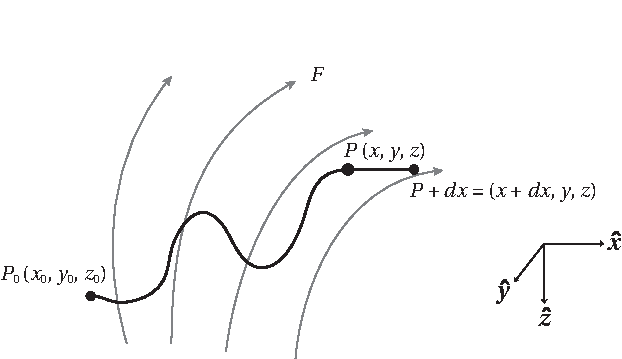
\includegraphics{potential/figures/work_path.pdf}
%     \caption{Path of a particle.}
%     \label{fig:path}
% \end{figure}

% Now lets suppose that we move our mass from $P_0$ starting at time $t_0$ and
% arrive at $P$ some time, $t$, later.  So lets integrate both sides with respect
% to time, which gives
% \begin{equation*}
%     \int_{t_0}^t \vb{F} \cdot \vb{v} \dd{t'} = K - K_0 .
% \end{equation*}
% We are going to do something a bit sneaky here and rewrite our integral in terms
% of space instead of time.  To do so, we need to change our limits of integration
% and our variable of integration.  We can relate the change in position
% $\dd{\vb{s}}$ to the change in time by $\dd{\vb{s}} = \vb{v} \dd{t'}$.  Just as velocity, 
% $\dd{\vb{s}}$ is a vector tangent to the path at all points.  This change in
% variables allows us to write
% \begin{equation*}
%     \int_{P_0}^P \vb{F} \cdot \dd{\vb{s}} = W(P,P_0) ,
% \end{equation*}
% where $W(P,P_0)$ is the work done in moving the mass from point $P_0$ to $P$.
% Note that we had to change from kinetic energy to work because our result is now
% independent of time.

% If the work done to move the test mass from $P_0$ to $P$ is independent of the
% path it takes to get the field is {\it conservative}.  While work is typically
% path-dependent, we will assume that for our purposes in this instance it is
% path-independent.  Lets add a third point a distance $\Delta x$ from $P$, $P +
% \Delta x$.  For a conservative field, the work done is path independent, hence,
% the work done moving from $P_0$ to $P$ and additionally from $P$ to $P + \Delta
% x$ must be the same as the work done in moving from $P_0$ to $P + \Delta x$,
% i.e.,
% \begin{equation*}
%     W(P,P_0) + W(P + \Delta x,P) = W(P + \Delta x,P_0) .
% \end{equation*}
% Our true interest is the incremental work required to move from $P$ to $P +
% \Delta x$, hence
% \begin{equation*}
%     W(P + \Delta x,P) = W(P + \Delta x,P_0) - W(P,P_0) .
% \end{equation*}
% Using our integral definition for a force we can write the above as
% \begin{equation*}
%     \int_{P}^{P + \Delta x} F_x(x,y,z) dx = W(P + \Delta x,P_0) - W(P,P_0) .
% \end{equation*}
% Dividing both sides by $\Delta x$ removes the integral.  According to the mean
% value theorem, mean of a function must fall on at least one point between the
% two end-points, which allows us to write the mean force in the $x$-direction as
% $F_x(x + \epsilon \Delta x,y,z)$ where $0 < \epsilon < 1$.  Hence,
% \begin{equation*}
%     F_x(x + \epsilon \Delta x,y,z) = \frac{W(P + \Delta x,P_0) - W(P,P_0)}{\Delta x} .
% \end{equation*}
% As $\Delta x \to 0$,
% \begin{equation*}
%     F_x(x,y,z) = \pdv{W}{x} .
% \end{equation*}
% If we apply the same logic to $y$- and $z$-directions, we find
% \begin{align*}
%     \vb{F}(x,y,z) & = \vu{x} \pdv{W}{x} + \vu{y} \pdv{W}{y} + \vu{z} \pdv{W}{z} ,\\
%     \vb{F} &= \grad W .
% \end{align*}

% Lets take this one step further.  Recall that a force is a scalar times a
% vector, $\vb{F} = m \vb{a}$, but lets make this general since we will not
% always discuss motion/gravity.  Sometimes we will be talking stresses in rocks (which
% act like springs), or forces on charged particles (electricity and magnetism).
% Therefore, lets instead write a force generally as a scalar constant, $b$, and a 
% vector field, $C$ (i.e., $\vb{F} = b \vb{C}$).  Let us then rewrite the result
% from our last step of our derivation above to give
% \begin{equation*}
%     b \vb{C} = b \grad (\phi) ,
% \end{equation*}
% where our work function $W$ is now written in terms of our generic scalar and a
% new scalar field, which we call the potential field, $\phi$.  We can now divide
% through by $b$ to achieve
% \begin{equation}
%     \vb{C} = \grad \phi .
% \end{equation}